\subsection{Temperature Analysis: The Role of $\beta$ in Gradient Flow}
\label{sec:temperature_analysis}

The temperature parameter $\beta$ in the hard concrete distribution plays a crucial role in determining the behavior of our Probabilistic Top-K SAE. Through systematic experiments across different sparsity levels ($K \in \{8, 16, 32\}$) and temperatures ($\beta \in \{0.5, 1.0, 5.0, 10.0\}$), we uncover important insights about the interplay between temperature, sparsity, and reconstruction quality.

\subsubsection{Temperature Effects on Reconstruction Quality}

Figure~\ref{fig:temperature_pareto} demonstrates that reconstruction quality is highly sensitive to the temperature parameter, particularly at low sparsity levels. At $K=8$, increasing $\beta$ from 0.5 to 5.0 reduces MSE by approximately 27\% (from 5.83 to 4.25 on layer 10). However, the benefits plateau beyond $\beta=5.0$, with minimal improvements observed at $\beta=10.0$.

\begin{figure}[t]
    \centering
    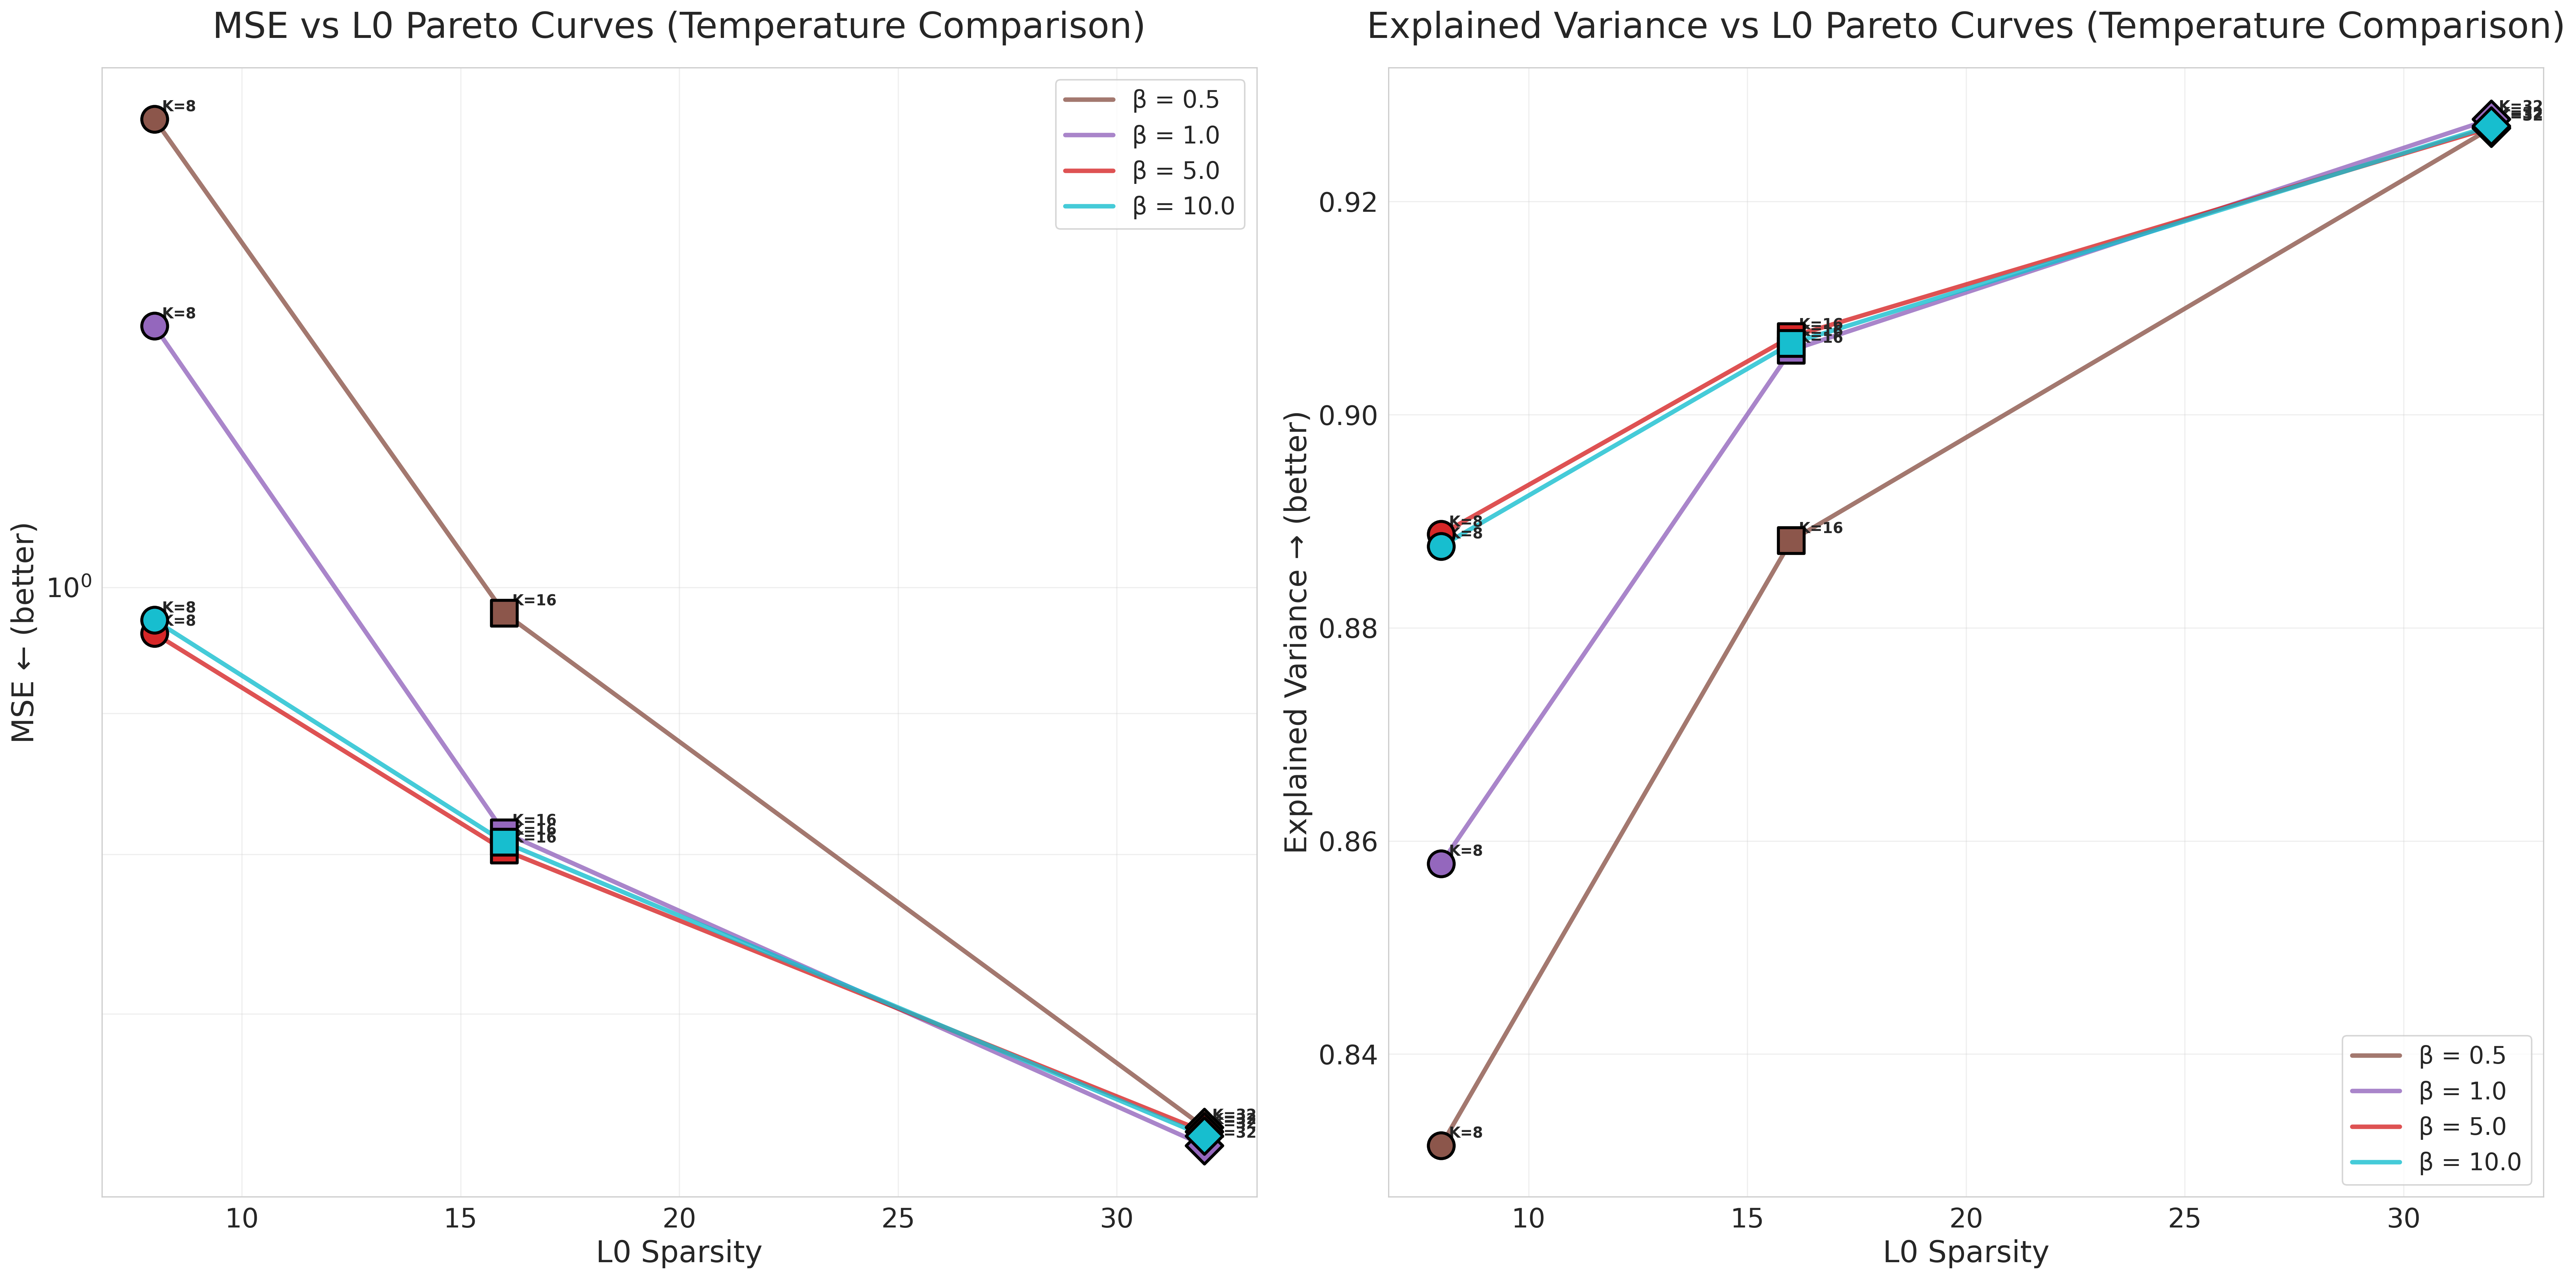
\includegraphics[width=\textwidth]{plots/temperature/temperature_pareto_curves_blocks_6_hook_resid_pre.png}
    \caption{Temperature Pareto curves showing MSE vs L0 sparsity (left) and Explained Variance vs L0 sparsity (right) for layer 6. Each curve represents a different temperature $\beta \in \{0.5, 1.0, 5.0, 10.0\}$ across sparsity levels $K \in \{8, 16, 32\}$. Higher temperatures (shown in red for $\beta=5$) consistently achieve better reconstruction quality.}
    \label{fig:temperature_pareto}
\end{figure}

The temperature effect diminishes as sparsity increases. At $K=32$, the performance gap between $\beta=0.5$ and $\beta=5.0$ narrows significantly, suggesting that higher sparsity naturally provides more gradient paths, reducing the importance of temperature-based smoothing.

\subsubsection{Understanding the Mechanism}

The hard concrete distribution samples gate values $z$ according to:
\begin{equation}
z = \sigma\left(\frac{1}{\beta}(\log u - \log(1-u) + \log \alpha)\right)
\end{equation}
where $u \sim \text{Uniform}(0,1)$ and $\alpha$ are the gate logits. Lower temperatures ($\beta < 1$) create sharper, more deterministic gates, while higher temperatures produce smoother, more stochastic gates.

At low temperatures, the gates become nearly binary during training, creating two problems:
\begin{enumerate}
    \item \textbf{Vanishing gradients}: Features with low gate values receive exponentially small gradients, preventing them from learning useful representations.
    \item \textbf{Feature collapse}: Once a feature's gate approaches zero, it rarely recovers, leading to many "dead" features.
\end{enumerate}

Higher temperatures address both issues by maintaining broader gradient flow during training. This is evidenced by the dramatic increase in alive dictionary components: at $K=8$, layer 6 shows 16,197 alive features with $\beta=5$ compared to only 4,715 with $\beta=0.5$.

\subsubsection{The Sparsity-Temperature Trade-off}

Our results reveal an important interaction between sparsity level and optimal temperature:

\paragraph{Low sparsity ($K=8$):} Higher temperatures are essential. The limited number of active features creates a severe gradient bottleneck that only smooth, stochastic gates can alleviate. The MSE improvement from $\beta=0.5$ to $\beta=5.0$ ranges from 25-43\% across layers.

\paragraph{Medium sparsity ($K=16$):} Temperature effects remain significant but less dramatic. The additional active features provide more gradient paths, partially compensating for sharp gates. MSE improvements are typically 10-20\%.

\paragraph{High sparsity ($K=32$):} Temperature becomes less critical. With many active features, gradient flow is naturally preserved. Performance differences between $\beta=1.0$ and $\beta=5.0$ are often negligible (<5\% MSE difference).

This pattern suggests that temperature acts as a regularizer that prevents premature feature specialization. At low sparsity, this regularization is crucial for exploration; at high sparsity, the abundance of active features naturally encourages exploration.

\subsubsection{Practical Implications}

Based on our analysis, we recommend:
\begin{itemize}
    \item Use $\beta \geq 5.0$ for all sparsity levels to ensure robust training
    \item Consider higher temperatures ($\beta \approx 10$) for extremely sparse regimes ($K < 8$)
    \item Avoid low temperatures ($\beta < 1.0$) which consistently underperform
\end{itemize}

The default $\beta=5.0$ emerges as a robust choice across all settings, providing near-optimal performance without requiring sparsity-specific tuning. This temperature strikes an effective balance between maintaining gradient flow and allowing features to specialize, making it suitable for practical applications where the optimal sparsity level may not be known a priori. 